\documentclass [10pt] {beamer}
\usetheme      {Madrid}
\usecolortheme {rose}
\usefonttheme  {serif}

\setbeamertemplate {navigation symbols} {}
\setbeamertemplate {footline} [page number]
\setbeamertemplate {caption} [numbered]
\setbeamertemplate {itemize items} [circle]
\setbeamertemplate {enumerate items} [square]
\setbeamertemplate {theorems} [numbered]

\setbeamercolor {footnote mark} {fg = red}
\setbeamercolor {block title} {fg = black}

\setbeamersize {text margin left=10pt, text margin right=10pt}

\usepackage [T2A] {fontenc}
\usepackage [utf8] {inputenc}
\usepackage [english] {babel}
\usepackage {mathrsfs}
\usepackage {graphicx}
\usepackage {ulem}
\usepackage {amssymb}
\usepackage {amsmath}
\usepackage {amsfonts}
\usepackage {amsthm}
\usepackage {indentfirst}
\usepackage {array}
\usepackage {multicol}

\newenvironment{psm}
	{\left( \begin{smallmatrix}}
	{\end{smallmatrix} \right) }

% \def\redlozenge{\mathbin{\color{red}\blacklozenge}}
% \begin{equation} ... \tag{$\redlozenge$} \end{equation}

\title{Coding of bounded solutions of equation $u_{xx} - u + \eta(x) u^3 = 0$ with periodic piecewise \\ constant function $\eta(x)$}

\author{\underline{M. E. Lebedev}, G. L. Alfimov \\ {\small MIET University, Zelenograd, Moscow, Russia}}
\date{Lake Bannoe \\ March, 2021}

\begin{document}

% ************
% * SLIDE 01 *
% ************
\begin{frame}
	\titlepage
\end{frame}

% ************
% * SLIDE 02 *
% ************
\begin{frame}
	\frametitle{Objective \& Motivation}
	\begin{columns}[T]
		\begin{column}{.5\textwidth}
			Our \underline{objective} is an equation
			\begin{equation}
				u_{xx} - u + \eta(x) u^3 = 0,
				\label{eq:main}
			\end{equation}
			$\eta(x)$ is a periodic piecewise-constant function of period $L = L_* + L_0$,
			\begin{equation*}
				\eta(x) = \left\{
					\begin{array}{rl}
						-1, &  x \in [0; L_*]; \\[1.5mm]
						a^2, & x \in [L_*; L_* + L_0],
					\end{array}
				\right.
			\end{equation*}
			where $a \in \mathbb{R}$.
			\begin{figure}
			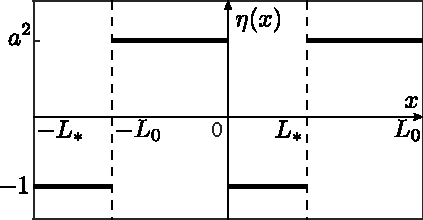
\includegraphics[width = 1\textwidth]{pic/piecewise-constant.pdf}
			\end{figure}
		\end{column}
		\hfill
		\begin{column}{.5\textwidth}
			Our \underline{motivation} is a GPE equation:
			\begin{equation}
				i \Psi_t + \Psi_{xx} + P(x) |\Psi|^2 \Psi = 0,
			\end{equation}
			$P(x) \in \mathbb{R}$ is a periodic function that changes its sing on the period.

			\vspace{10pt}
			
			Stationary states equation:
			\begin{equation*}
				u_{xx} + \omega u + P(x) u^3 = 0, \quad \omega < 0.
			\end{equation*}
			We wrote a paper!
			\begin{figure}
			\includegraphics[width = 1\textwidth]{pic/publication.png}
			\end{figure}
			
			Many localised stationary states was found (numerically).
		\end{column}
	\end{columns}
\end{frame}

% ************
% * SLIDE .. *
% ************
\begin{frame}
	\begin{center}
		{\Huge Part I.} \\[10pt] {\LARGE Common sense}
	\end{center}
\end{frame}

% ************
% * SLIDE .. *
% ************
\begin{frame}
	\frametitle{Phase portraits}
	\begin{columns}[T]
		\begin{column}{.5\textwidth}
			$\mathcal{P}_*$ mapping:
			\begin{figure}
			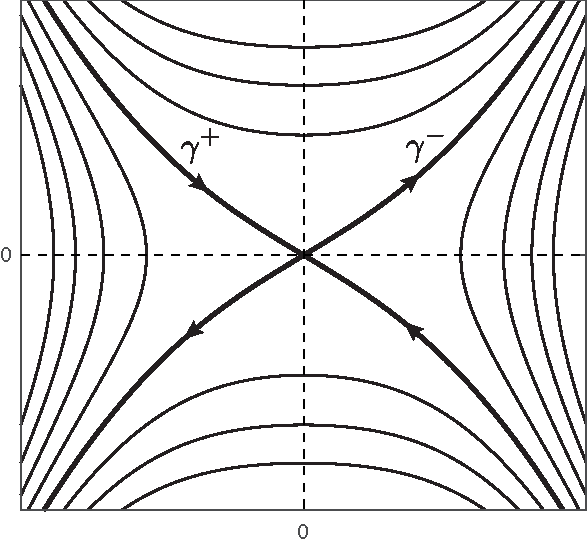
\includegraphics[width = 0.9\textwidth]{pic/phase-portrait-1.pdf}
			\caption{Phase portrait for the equation $u_{xx} - u - u^3 = 0$.}
			\label{pic:phase-portrait-1}
			\end{figure}
		\end{column}
		\hfil
		\begin{column}{.5\textwidth}
			$\mathcal{P}_0$ mapping:
			\begin{figure}
			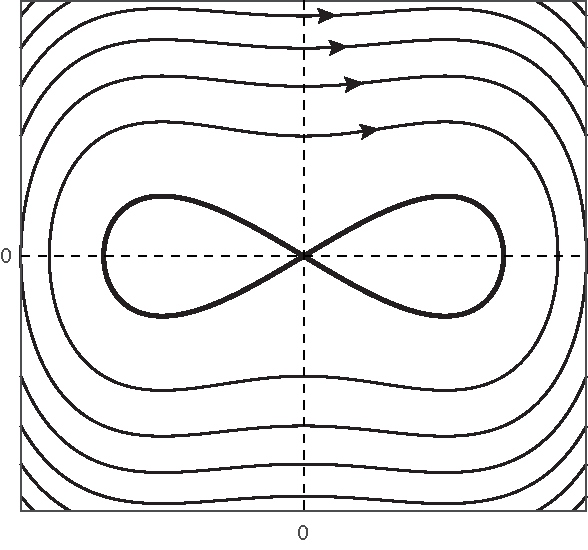
\includegraphics[width = 0.9\textwidth]{pic/phase-portrait-2.pdf}
			\caption{Phase portrait for the equation $u_{xx} - u + u^3 = 0$.}
			\label{pic:phase-portrait-2}
			\end{figure}
		\end{column}
	\end{columns}
	
	Poincar\'e map $\mathcal{P}(u_0, u_0') = (u(L), u'(L))$, $u(x)$ is a solution of \eqref{eq:main} with initial conditions $(u_0, u_0')$; $\mathcal{P} = \mathcal{P}_0 \mathcal{P}_*$.
\end{frame}

% ************
% * SLIDE .. *
% ************
\begin{frame}
	\begin{center}
		{\Huge Part II.} \\[10pt] {\LARGE Poincar\'e map}
	\end{center}
\end{frame}

% ************
% * SLIDE .. *
% ************
\begin{frame}
	\frametitle{$\textrm{dom}(\mathcal{P_*}) = \mathscr{U}_{L_*}^+$}
	\begin{columns}[T]
		\begin{column}{.5\textwidth}
			\begin{figure}
			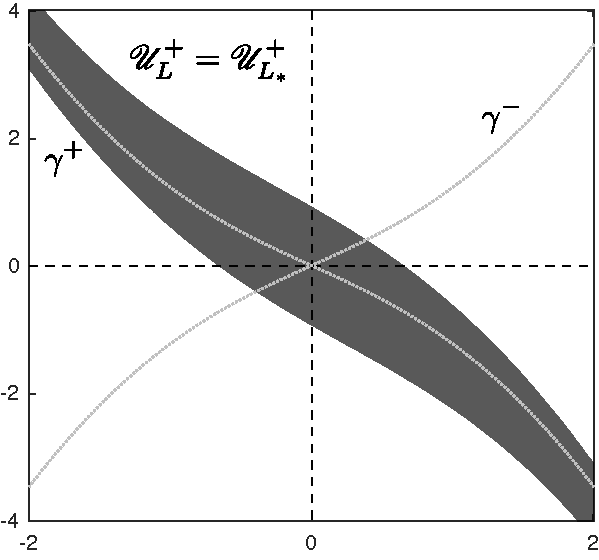
\includegraphics[width = 1\textwidth]{pic/h-strips-step-1.pdf}
			\caption{Domain of $\mathcal{P}$ for the parameters $(L_*, L_0, a) = (2, 1, 1)$; $\gamma^{\pm}$ are separatrices for the equation $u_{xx} - u - u^3 = 0$.}
			\label{pic:h-striprs-step-1}
			\end{figure}
		\end{column}
		\begin{column}{.5\textwidth}
			\begin{theorem}
				$\forall L_*, \, 0 < L_* < +\infty$, set $\mathscr{U}_{L_*}^+$ is an infinite curvilinear open strip, that
				\begin{enumerate}
					\item[(a)] $\mathscr{U}_{L_*}^+$ is symmetric with respect to the origin and contains $\gamma^+$;
					\item[(b)] $\mathscr{U}_{L_*}^+$ is bounded by two symmetric monotonically decreasing curves (which are $C^1$ functions);
					\item[(c)] vertical dimension of the $\mathscr{U}_{L_*}^+$ tends to zero exponentially when $L_* \to +\infty$.
				\end{enumerate}
			\end{theorem}
			\begin{align*}
				\mathscr{U}_L^+ & \equiv \textrm{dom}(\mathcal{P}) = \textrm{dom}(\mathcal{P}_0 \mathcal{P}_*) \\
				& = \textrm{dom}(\mathcal{P}_*) \equiv \mathscr{U}_{L_*}^+.
			\end{align*}
		\end{column}
	\end{columns}
\end{frame}

% ************
% * SLIDE .. *
% ************
\begin{frame}
	\frametitle{$\mathcal{P}_*(\mathscr{U}_L^+) = \mathscr{U}_{L_*}^-$}
	\begin{columns}[T]
		\begin{column}{.5\textwidth}
			\begin{figure}
			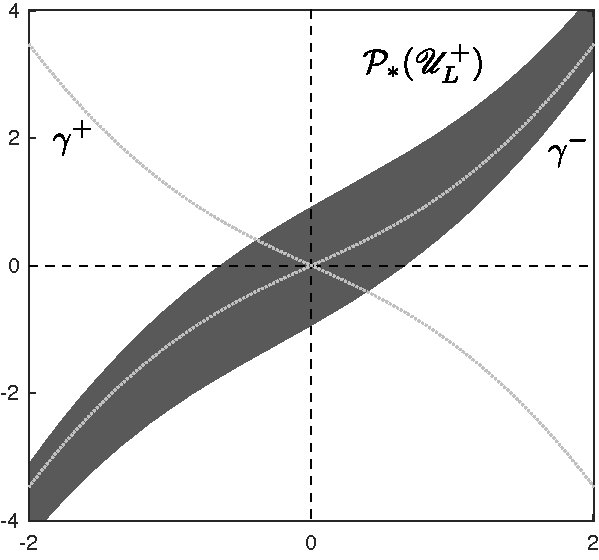
\includegraphics[width = 1\textwidth]{pic/h-strips-step-2.pdf}
			\caption{$\mathcal{P}_*$--image of $\mathscr{U}_L^+$ for the parameters $(L_*, L_0, a) = (2, 1, 1)$.}
			\label{pic:h-striprs-step-2}
			\end{figure}
		\end{column}
		\begin{column}{.5\textwidth}
			\begin{theorem}
				$\forall L_*, \, 0 < L_* < +\infty$, set $\mathscr{U}_{L_*}^-$ is an infinite curvilinear open strip, that
				\begin{enumerate}
					\item[(a)] $\mathscr{U}_{L_*}^-$ is symmetric with respect to the origin and contains $\gamma^-$;
					\item[(b)] $\mathscr{U}_{L_*}^-$ is bounded by two symmetric monotonically increasing curves (which are $C^1$ functions);
					\item[(c)] vertical dimension of the $\mathscr{U}_{L_*}^-$ tends to zero exponentially when $L_* \to +\infty$.
				\end{enumerate}
			\end{theorem}
			\begin{equation*}
				\mathcal{P}_*(\mathscr{U}_L^+) = I \mathscr{U}_L^+,
			\end{equation*}
			where $I$ is a reflection with respect to the $u$ axis on the phase plane $(u, u')$.
		\end{column}
	\end{columns}
\end{frame}

% ************
% * SLIDE .. *
% ************
\begin{frame}
	\frametitle{$\mathcal{P}_0(\gamma_-)$}
	\begin{columns}[T]
		\begin{column}{.5\textwidth}
			\begin{figure}
			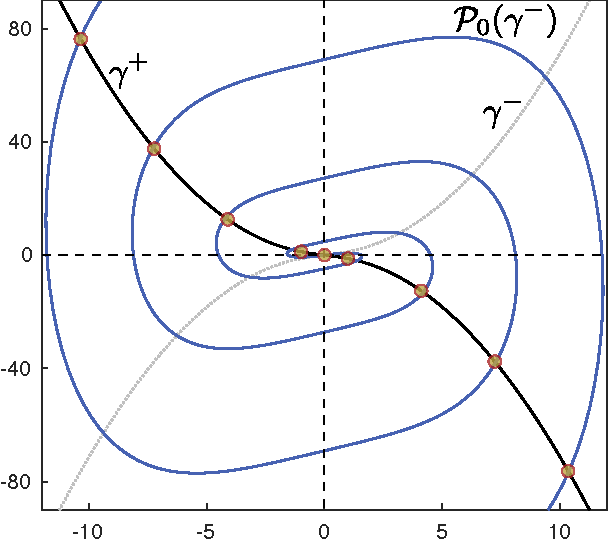
\includegraphics[width = 1\textwidth]{pic/map-of-separatrix.pdf}
			\caption{$\mathcal{P}_0(\gamma^-)$ (solid blue line) is an infinite spiral; yellow dots are the points of intersections $\mathcal{P}_0(\gamma^-) \cap \gamma^+$ predicted by the equation \eqref{eq:intersections}.}
			\label{pic:map-of-separatrix}
			\end{figure}
		\end{column}
		\begin{column}{.5\textwidth}
			\begin{theorem}
				$\mathcal{P}_0$--image of the curve $\gamma^-$ is an infinite spiral, it intersects $\gamma^+$ infinitely many times at the points $\{0\} \cup \{u_{\pm n}\}$, where
				\begin{equation}
					u_{\pm n} = \pm \dfrac{2 a^{3/2} x_{n - 1}}{\sqrt[4]{a^2 + 1}} L_0^{
					-1} + O(L_0);
					\label{eq:intersections}
				\end{equation}
				$L_0  \to 0$, and $x_n$ are determined as
				\begin{equation*}
					x_n = \textrm{cn}^{-1} \left(\dfrac{\sqrt{a}}{\sqrt[4]{a^2 + 1}}, k\right) + \textrm{K}(k)n,
				\end{equation*}
				where $k = 1/\sqrt{2}$, $n \in \mathbb{N}$.
			\end{theorem}
			
			Here $\textrm{K}(\cdotp)$ is the complete elliptic integral of the 1st kind, $\textrm{cn}^{-1}$ is an inverse elliptic cosine.
		\end{column}
	\end{columns}
\end{frame}

% ************
% * SLIDE .. *
% ************
\begin{frame}
	\frametitle{$\mathcal{P}_0(\mathscr{U}_{L_*}^-) = \mathscr{U}_L^-$}
	\begin{columns}[T]
		\begin{column}{.5\textwidth}
			\begin{figure}
			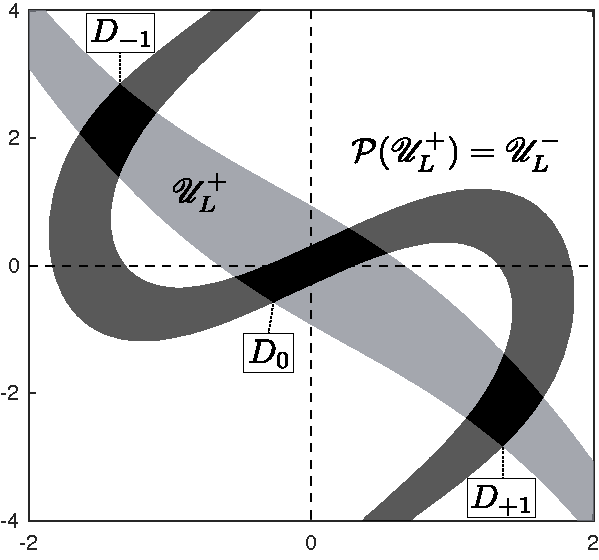
\includegraphics[width = 1\textwidth]{pic/h-strips-step-3.pdf}
			\caption{Three components $D_{-1}$, $D_0$, $D_{+1}$ (black) of the set $\mathscr{U}_L = \mathscr{U}_L^+ \cap \mathscr{U}_L^-$.}
			\label{pic:h-strips-step-3}
			\end{figure}
		\end{column}
		\begin{column}{.5\textwidth}
			\begin{equation*}
				\mathscr{U}_L^- \equiv \textrm{dom}(\mathcal{P}^{-1}) = \mathcal{P}_0 (\mathscr{U}_{L_*}^-) = \mathcal{P}(\mathscr{U}_L^-).
			\end{equation*}
			\begin{itemize}
				\item Both $\mathcal{P}$ and $\mathcal{P}^{-1}$ are defined on $\mathscr{U}_L = \mathscr{U}_L^+ \cap \mathscr{U}_L^-$. \\[10pt]
				\item $\mathscr{U}_L$ consists  of infinite number of components $\mathscr{U}_L = \bigcup_{i \in S} D_i$. \\[10pt]
				\item Each component except of the central one ($D_0$) is a curvilinear quadrangle with monotonic boarders ({\it island}). \\[10pt]
				\item $D_0$ can be made an {\it island} by varying parameters $(L_*, L_0, a)$.
			\end{itemize}
		\end{column}
	\end{columns}
\end{frame}

% ************
% * SLIDE .. *
% ************
\begin{frame}
	\frametitle{$\mathcal{P}(\mathscr{U}_L) = \bigcup_{i \in S} \mathcal{P}(D_i)$}
	\begin{columns}[T]
		\begin{column}{.5\textwidth}
			\begin{figure}
			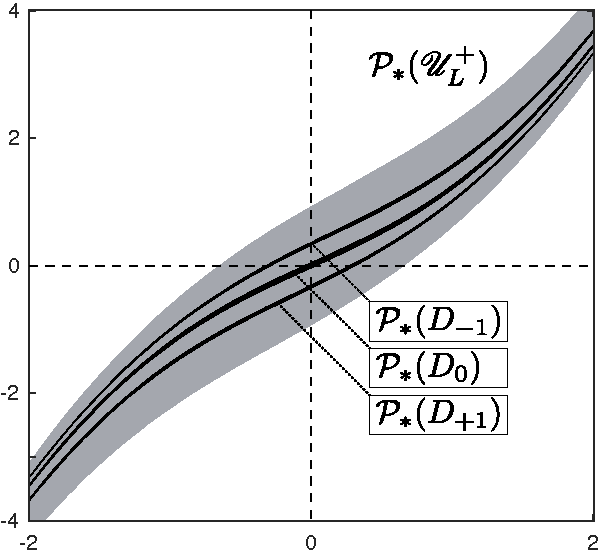
\includegraphics[width = 1\textwidth]{pic/h-strips-step-4.pdf}
			\caption{$\mathcal{P}_*$--image of the components $D_{-1}$, $D_0$, $D_{+1}$ of $\mathscr{U}_L$.}
			\label{pic:h-strips-step-4}
			\end{figure}
		\end{column}
		\begin{column}{.5\textwidth}
			\begin{figure}
			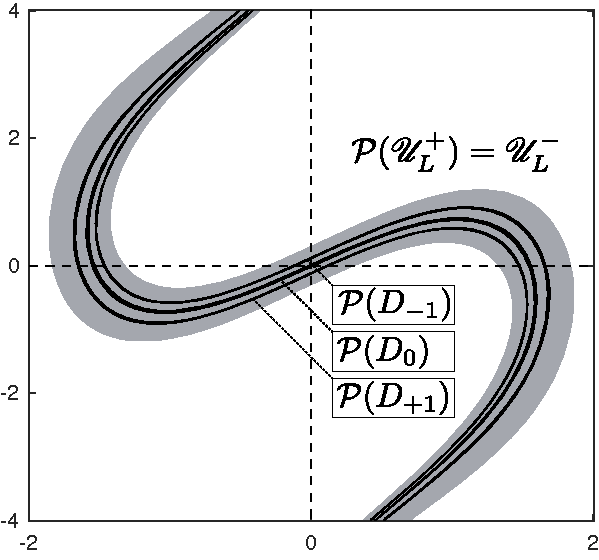
\includegraphics[width = 1\textwidth]{pic/h-strips-step-5.pdf}
			\caption{$\mathcal{P}$--image of the components $D_{-1}$, $D_0$, $D_{+1}$ of $\mathscr{U}_L$.}
			\label{pic:h-strips-step-5}
			\end{figure}
		\end{column}
	\end{columns}
\end{frame}

% ************
% * SLIDE .. *
% ************
\begin{frame}
	\frametitle{$\bigcup_{i \in S} \mathcal{P}(D_i) \cap \mathscr{U}_L$}
	\begin{columns}[T]
		\begin{column}{.5\textwidth}
			\begin{figure}
			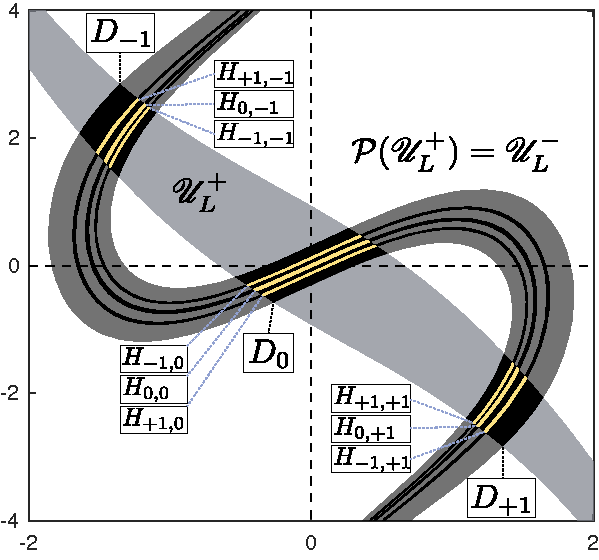
\includegraphics[width = 1\textwidth]{pic/h-strips-step-6.pdf}
			\caption{$h$-strips (yellow) as a result of intersections of $\mathcal{P}(D_i)$ and $\mathscr{U}_L$ sets for the components $D_{-1}$, $D_0$, $D_{+1}$.}
			\label{pic:h-strips-step-6}
			\end{figure}
		\end{column}
		\begin{column}{.5\textwidth}
			\begin{equation*}
				\forall i, j, \, H_{i, j} = \mathcal{P}(D_i) \cap D_j \neq \varnothing.
			\end{equation*}
			\begin{itemize}
				\item We call such sets as $h$-strips.\\[10pt]
				\item Here $h$-strips consist of points where both $\mathcal{P}$ and $\mathcal{P}^{-2}$ are defined.\\[10pt]
				\item This process can be continued, one can get points of initial condition where higher order of $\mathcal{P}^{-k}$ are defined.\\[10pt]
				\item Continuation of the process results in sets of nested $h$-strips.\\[10pt]
			\end{itemize}
		\end{column}
	\end{columns}
\end{frame}

% ************
% * SLIDE .. *
% ************
\begin{frame}
	\frametitle{$\bigcup_{i \in S} \mathcal{P}^{-1}(D_i) \cap \mathscr{U}_L$}
	\begin{columns}[T]
		\begin{column}{.5\textwidth}
			\begin{figure}
			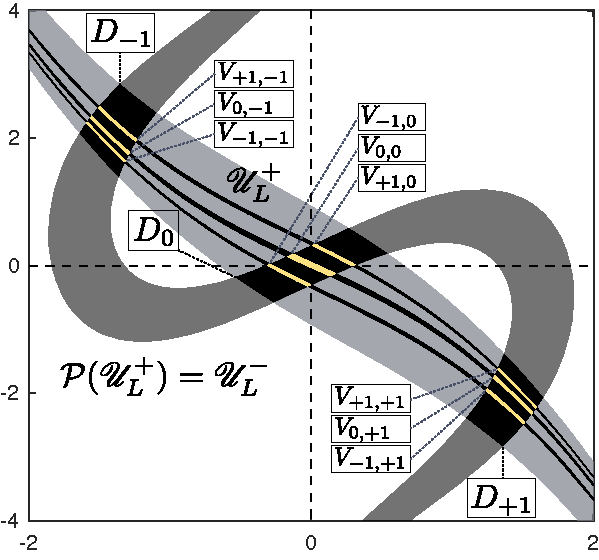
\includegraphics[width = 1\textwidth]{pic/v-strips-last-step.pdf}
			\caption{$v$-strips (yellow) as a result of intersections of $\mathcal{P}^{-1}(D_i)$ and $\mathscr{U}_L$ sets for the components $D_{-1}$, $D_0$, $D_{+1}$.}
			\label{pic:v-strips-last-step}
			\end{figure}
		\end{column}
		\begin{column}{.5\textwidth}
			\begin{equation*}
				\forall i, j, \, V_{i, j} = \mathcal{P}^{-1}(D_i) \cap D_j \neq \varnothing.
			\end{equation*}
			\begin{itemize}
				\item We call such sets as $v$-strips.\\[10pt]
				\item Here $v$-strips consist of points where both $\mathcal{P}^2$ and $\mathcal{P}^{-1}$ are defined.\\[10pt]
				\item This process can be continued, one can get points of initial condition where higher order of $\mathcal{P}^{k}$ are defined.\\[10pt]
				\item Continuation of the process results in sets of nested $v$-strips.\\[10pt]
			\end{itemize}
		\end{column}
	\end{columns}
\end{frame}

% ************
% * SLIDE .. *
% ************
\begin{frame}
	\frametitle{All together}
	\begin{columns}[T]
		\begin{column}{.5\textwidth}
			\begin{figure}
			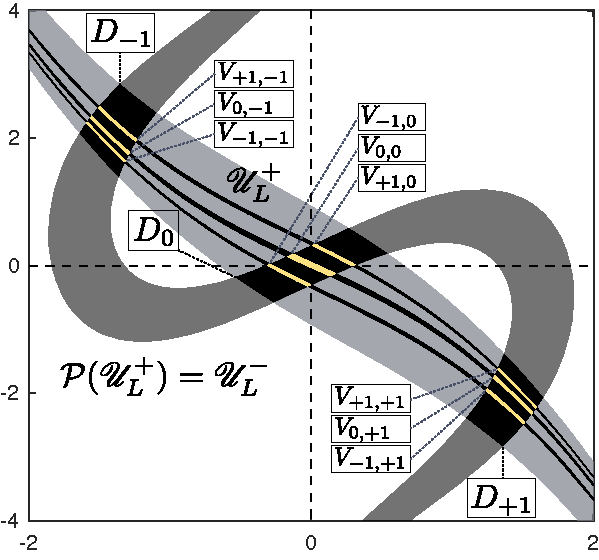
\includegraphics[width = 1\textwidth]{pic/v-strips-last-step.pdf}
			\caption{$v$-strips (yellow) as a result of intersections of $\mathcal{P}^{-1}(D_i)$ and $\mathscr{U}_L$ sets for the components $D_{-1}$, $D_0$, $D_{+1}$.}
			\label{pic:v-strips-last-step}
			\end{figure}
		\end{column}
		\begin{column}{.5\textwidth}
			\begin{figure}
			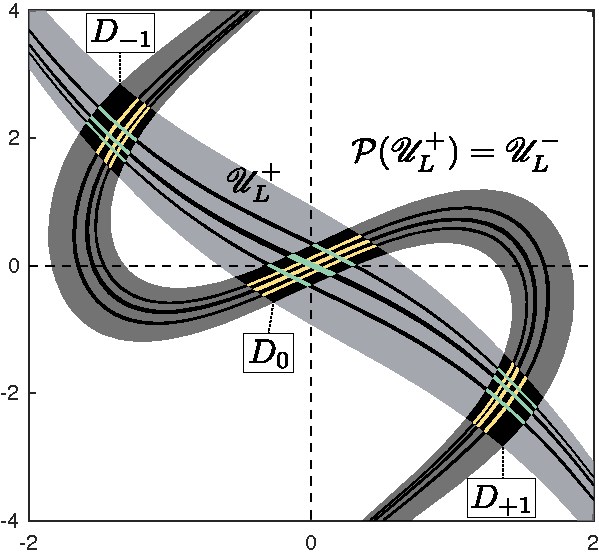
\includegraphics[width = 1\textwidth]{pic/h-and-v-strips.pdf}
			\caption{Intersections of $h$ and $v$-strips (yellow and green) consist of points where both $\mathcal{P}^2$ and $\mathcal{P}^{-2}$ are defined.}
			\label{pic:h-and-v-strips}
			\end{figure}
		\end{column}
	\end{columns}
\end{frame}

% ************
% * SLIDE .. *
% ************
\begin{frame}
	\begin{center}
		{\Huge Part III.} \\[10pt] {\LARGE Solutions coding}
	\end{center}
\end{frame}

% ************
% * SLIDE .. *
% ************
\begin{frame}
	\frametitle{$\mathcal{O} \to \mathcal{S}_{\infty}$}
	\begin{columns}[T]
		\begin{column}{.5\textwidth}
			{\it Orbit} is a sequence of points $\{p_n\}$, that
			\begin{equation*}
				\mathcal{P}(p_n) = p_{n+1}.
			\end{equation*}
			
			$\mathcal{O}$ -- set of orbits of {\it regular} solution for the equation \eqref{eq:main}.

			\vspace{10pt}

			$\mathcal{S}$ -- set of bi-infinite sequences over the infinite alphabet 
			
			\begin{equation*}
				\{\dots, i_{-1}, i_0, i_1, \dots\},
			\end{equation*}
			where each symbol corresponds to the connected component $D_i \in \mathscr{U}_L$.
		
			\begin{center}
				It's easy to assign a {\it code} to the solution!
			\end{center}
		\end{column}
		\begin{column}{.5\textwidth}
			\begin{figure}
			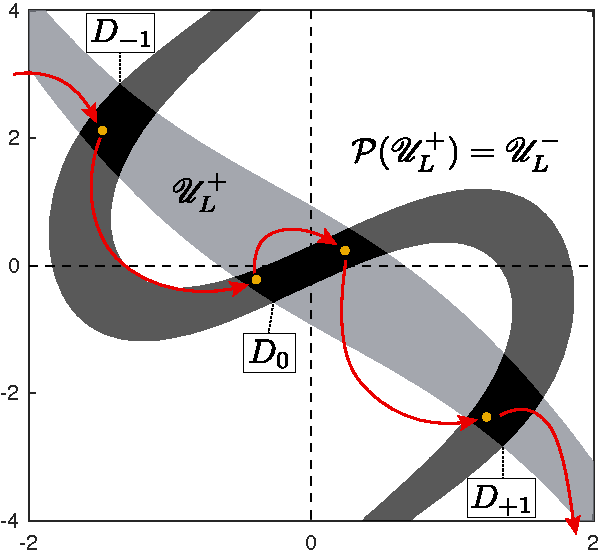
\includegraphics[width = 1\textwidth]{pic/orbit-on-a-phase-plane.pdf}
			\caption{Sketch of an orbit of a {\it regular} solution (yellow dots) that corresponds to the code sequence $\{\dots, -1, 0, 0, +1, \dots\}$.}
			\end{figure}
		\end{column}
	\end{columns}
\end{frame}

% ************
% * SLIDE .. *
% ************
\begin{frame}
	\frametitle{Solutions and their codes}
	\begin{columns}[T]
		\begin{column}{.5\textwidth}
			\begin{figure}
			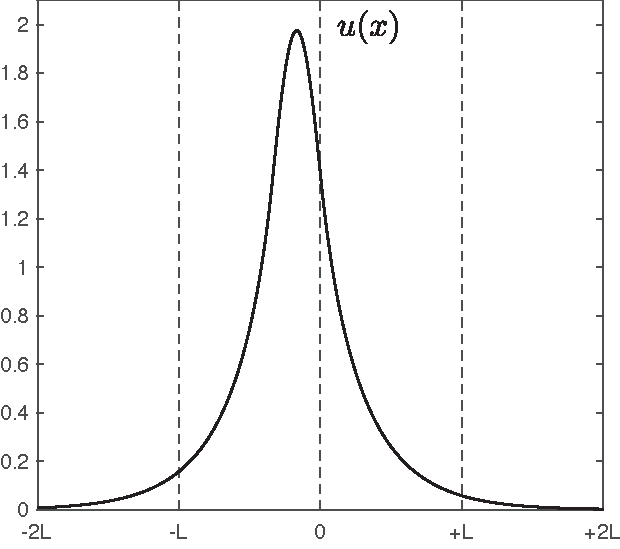
\includegraphics[width = 1\textwidth]{pic/solution-1.pdf}
			\caption{Solution of the code $\{\dots, 0, 0, +1,  0, 0, \dots\}$.}
			\end{figure}
		\end{column}
		\begin{column}{.5\textwidth}
			\begin{figure}
			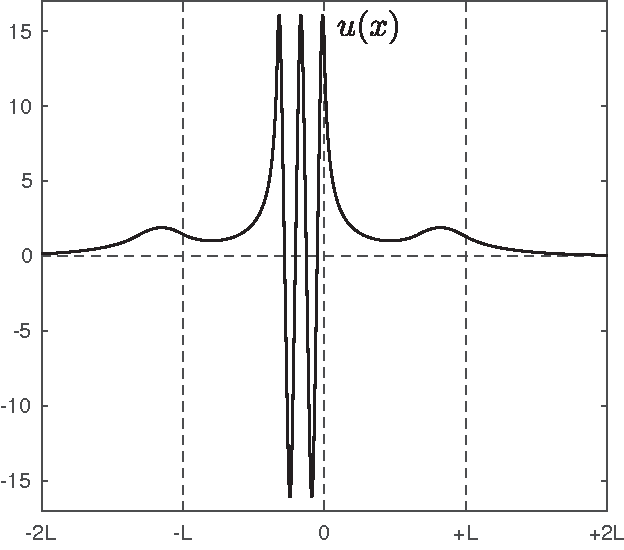
\includegraphics[width = 1\textwidth]{pic/solution-2.pdf}
			\caption{Solution of the code $\{\dots, 0, +1, +3, +1, 0, \dots\}$.}
			\end{figure}
		\end{column}
	\end{columns}
\end{frame}

% ************
% * SLIDE .. *
% ************
\begin{frame}
	\frametitle{Solutions and their codes}
	\begin{columns}[T]
		\begin{column}{.5\textwidth}
			\begin{figure}
			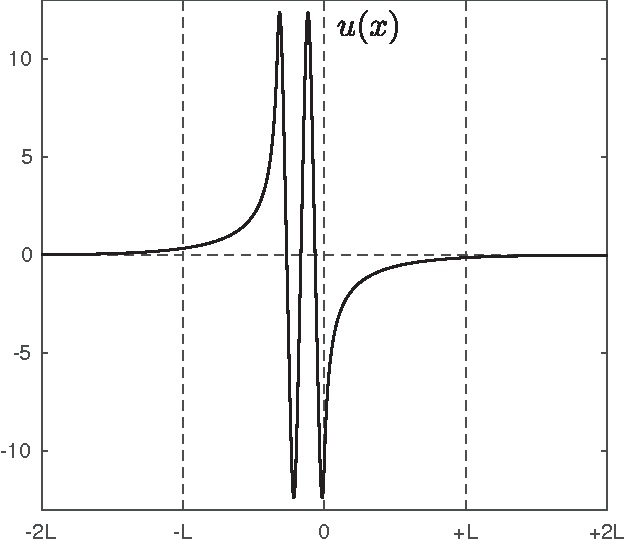
\includegraphics[width = 1\textwidth]{pic/solution-3.pdf}
			\caption{Solution of the code $\{\dots, 0, 0, -3, 0, 0, \dots\}$.}
			\end{figure}
		\end{column}
		\begin{column}{.5\textwidth}
			\begin{figure}
			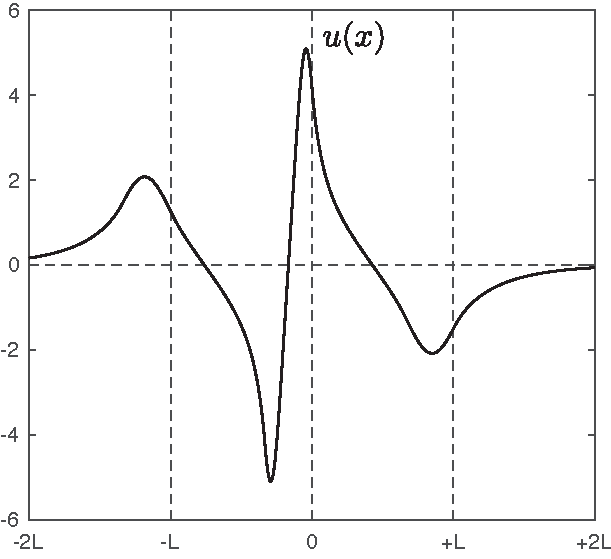
\includegraphics[width = 1\textwidth]{pic/solution-4.pdf}
			\caption{Solution of the code $\{\dots, 0, +1, +2, -1, 0, \dots\}$.}
			\end{figure}
		\end{column}
	\end{columns}
\end{frame}

% ************
% * SLIDE .. *
% ************
\begin{frame}
	\frametitle{$\mathcal{S}_{\infty} \to \mathcal{O}$?}
	By code $\{\dots, i_{-1}, i_0, i_1, \dots\}$ find initial conditions for the equation \eqref{eq:main} whose orbit visit components of $\mathscr{U}_L$ in a right order ($X \xrightarrow{\mathcal{P}} Y = \mathcal{P}(X) \cap Y$).
	\begin{columns}[T]
		\begin{column}{.5\textwidth}
			\begin{alignat*}{2}
				& D_{i_0} \supseteq H_{i_0} & = & D_{i_0}; \\[3pt]
				& D_{i_0} \supseteq H_{i_{-1}, i_0} & = & D_{i_{-1}} \xrightarrow{\mathcal{P}} D_{i_0}; \\[3pt]
				& D_{i_0} \supseteq H_{i_{-2}, i_{-1}, i_0} & = & D_{i_{-2}} \xrightarrow{\mathcal{P}} D_{i_{-1}} \xrightarrow{\mathcal{P}} D_{i_0}; \\[3pt]
				& \dots.
			\end{alignat*}
			Nested $h$-strips $\{H_n\}$:
			$$\cdots \subseteq H_{i_{-2}, i_{-1}, i_0} \subseteq H_{i_{-1}, i_0} \subseteq H_{i_0} = D_{i_0}.$$ 
			$$\{ H_n \} \xrightarrow{n \to \infty} h?$$
		\end{column}
		\hfill
		\begin{column}{.5\textwidth}
			\begin{alignat*}{2}
				& D_{i_0} \supseteq V_{i_0} & = & D_{i_0}; \\[2pt]
				& D_{i_0} \supseteq V_{i_1, i_0} & = & D_{i_1} \xrightarrow{\mathcal{P}^{-1}} D_{i_0}; \\[2pt]
				& D_{i_0} \supseteq V_{i_2, i_1, i_0} & = & D_{i_2} \xrightarrow{\mathcal{P}^{-1}} D_{i_1} \xrightarrow{\mathcal{P}^{-1}} D_{i_0}; \\[2pt]
				& \dots.
			\end{alignat*}
			Nested $v$-strips $\{V_n\}$:
			\begin{equation*}
				\cdots \subseteq V_{i_2, i_1, i_0} \subseteq V_{i_1, i_0} \subseteq V_{i_0} = D_{i_0}	
			\end{equation*}
			\begin{equation*}
				\{ V_n \} \xrightarrow{n \to \infty} v?		
			\end{equation*}
		\end{column}
	\end{columns}
	\vspace{10pt}
	\begin{center}
		Initial conditions in $D_{i_0}$ should belongs to the intersection $h \cap v$.
	\end{center}
\end{frame}

% ************
% * SLIDE .. *
% ************
\begin{frame}
	\begin{center}
		{\Huge Part IV.} \\[10pt] {\LARGE Uniqueness}
	\end{center}
\end{frame}

% ************
% * SLIDE .. *
% ************
\begin{frame}
	\frametitle{What is $h \cap v$?}
	\begin{theorem}
		Let
		\begin{itemize}
			\item all $\{H_n\}$ have monotone increasing / decreasing borders  which are graphs of $\gamma$-Lipschitz functions, and $\rho(H_{n+1}) \le (1 / \mu) \rho(H_n)$, $\mu > 1$;
			\item all $\{V_n\}$ have monotone decreasing / increasing borders  which are graphs of $\gamma$-Lipschitz functions,  and $\rho(V_{n+1}) \le (1 / \nu) \rho(V_n)$, $\nu > 1$;
		\end{itemize}
 		then the intersection $h \cap v$ consists of just one point!
		\end{theorem}
	\begin{columns}[T]
		\begin{column}{.4\textwidth}
		\begin{center}
			Here $\rho(\cdot)$ is a vertical (for $H_n$) or horizontal (for $V_n$) width of the strips.
		\end{center}
		\end{column}
		\begin{column}{.6\textwidth}
			\begin{figure}
			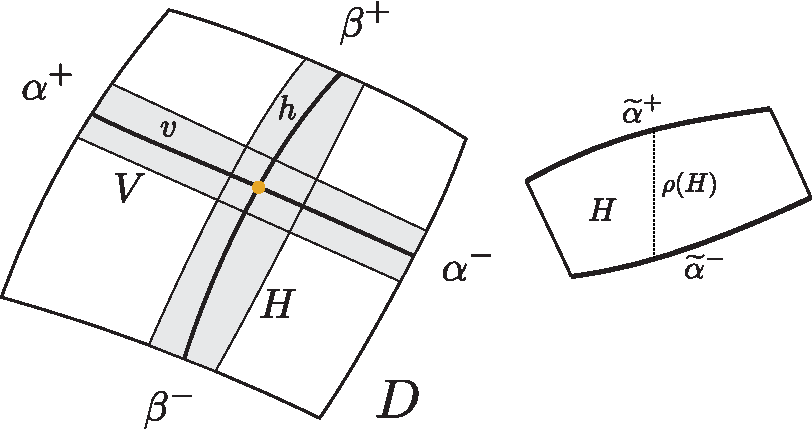
\includegraphics[width = 1\textwidth]{pic/curves-strips-width.pdf}
			\label{pic:curves-strips-width}
			\end{figure}
		\end{column}
	\end{columns}
\end{frame}

% ************
% * SLIDE .. *
% ************
\begin{frame}
	\frametitle{$D \mathcal{P}_p$, $D \mathcal{P}_p^{-1}$}
	\begin{columns}[T]
		\begin{column}{.5\textwidth}
			\begin{figure}
			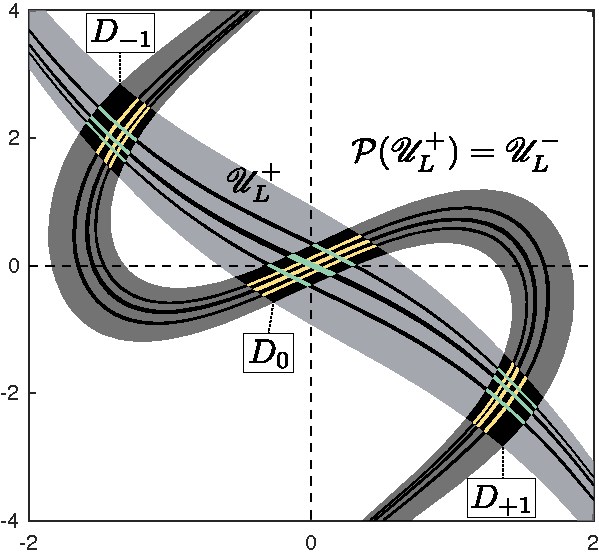
\includegraphics[width = 1\textwidth]{pic/h-and-v-strips.pdf}
			\caption{$H_{i,j}$ (yellow) and $V_{i,j}$ (green) are the points of interest.}
			\end{figure}
		\end{column}
		\begin{column}{.5\textwidth}
			\vspace{50pt}
			
			$D \mathcal{P}_p$ -- linearisation of the map $\mathcal{P}$ at the point $p$; $D \mathcal{P}_p^{-1}$  -- its inverse.
			
			\vspace{10pt}
			
			If linear operators $D \mathcal{P}_p$, $D \mathcal{P}_p^{-1}$ satisfy some restrictions then the conditions of the above mentioned theorem are valid!
		\end{column}
	\end{columns}
\end{frame}

% ************
% * SLIDE .. *
% ************
\begin{frame}
	\frametitle{Theorem about $h$-strips mapping}
	\begin{theorem}[About $h$-strips mapping]
		Let Poincar\'e map $\mathcal{P}$ and its inverse $\mathcal{P}^{-1}$ are defined on an island set $\bigcup_{i \in S} D_i$, where $S$ -- set of indices, $\forall i, j \in S$ set $V_{j,i} = \mathcal{P}^{-1} D_j \cap D_i$ is non-empty, $\mathcal{P}$ is defined on the closure $\overline{V_{j,i}}$, and one the following conditions held:
		\begin{enumerate}
			\item[(1)] borders $\alpha_i^{\pm}$ of an island $D_i$ are increasing curves, $\forall p \in \overline{V_{j,i}}$ signs of the operator $D \mathcal{P}_p = (a_{mn})$ have exactly one of the following configurations:
				\begin{center}
					(a) $\begin{psm} + & + \\ + & + \end{psm}$, \quad
					(b) $\begin{psm} - & - \\ - & - \end{psm}$, \quad
					(c) $\begin{psm} + & + \\ - & - \end{psm}$, \quad
					(d) $\begin{psm} - & - \\ + & + \end{psm}$;
				\end{center}
				borders $\alpha_j^{\pm}$ of $D_j$ are increasing for (a), (b), and decreasing for (c), (d);
			\item[(2)] borders $\alpha_i^{\pm}$ of an island $D_i$ are decreasing curves, $\forall p \in \overline{V_{j,i}}$ signs of the operator $D \mathcal{P}_p = (a_{mn})$ 	have exactly one of the following configurations:
				\begin{center}
					(a) $\begin{psm} + & - \\ - & + \end{psm}$, \quad
					(b) $\begin{psm} - & + \\ + & - \end{psm}$,	\quad
					(c) $\begin{psm} + & - \\ + & - \end{psm}$, \quad
					(d) $\begin{psm} - & + \\ - & + \end{psm}$;		
				\end{center}
				borders $\alpha_j^{\pm}$ of $D_j$ are decreasing for (a), (b), and increasing for (c), (d);
		\end{enumerate}
		and moreover $\exists \mu > 1$ such that $\forall p \in \overline{V_{j,i}}$, $|a_{11}| \ge \mu$, then for any monotone $h$-strip $H \in D_i$, $\forall j \in S$, $\mathcal{P} H \cap D_j = \widetilde{H}_j$ is also a monotone $h$-strip, and $\rho(\widetilde{H}_j) \le (1 / \mu) \rho(H)$.
\end{theorem}
\end{frame}

% ************
% * SLIDE .. *
% ************
\begin{frame}
	\frametitle{Theorem about $v$-strips mapping}
	\begin{theorem}[About $v$-strips mapping]
		Let Poincar\'e map $\mathcal{P}$ and its inverse $\mathcal{P}^{-1}$ are defined on an island set $\bigcup_{i \in S} D_i$, where $S$ -- set of indices, $\forall i, j \in S$ set $H_{i,j} = \mathcal{P} D_i \cap D_j$ is non-empty, $\mathcal{P}^{-1}$ is defined on the closure $\overline{H_{i,j}}$, and one the following conditions held:
		\begin{enumerate}
			\item[(1)] borders $\beta_i^{\pm}$ of an island $D_i$ are increasing curves, $\forall p \in \overline{H_{i,j}}$ signs of the operator $D \mathcal{P}_0^{-1} = (b_{mn})$ have exactly one of the following configurations:
				\begin{center}
					(a) $\begin{psm} + & + \\ + & + \end{psm}$, \quad
					(b) $\begin{psm} - & - \\ - & - \end{psm}$, \quad
					(c) $\begin{psm} + & + \\ - & - \end{psm}$, \quad
					(d) $\begin{psm} - & - \\ + & + \end{psm}$;
				\end{center}
				borders $\beta_j^{\pm}$ of $D_j$ are increasing for (a), (b), and decreasing for (c), (d);
			\item[(2)] borders $\beta_i^{\pm}$ of an island $D_i$ are decreasing curves, $\forall p \in \overline{H_{i,j}}$ signs of the operator $D \mathcal{P}_0^{-1} = (b_{mn})$ have exactly one of the following configurations:
				\begin{center}
					(a) $\begin{psm} + & - \\ - & + \end{psm}$, \quad
					(b) $\begin{psm} - & + \\ + & - \end{psm}$, \quad
					(c) $\begin{psm} + & - \\ + & - \end{psm}$, \quad
					(d) $\begin{psm} - & + \\ - & + \end{psm}$;
				\end{center}
				borders $\beta_j^{\pm}$ of $D_j$ are decreasing for (a), (b), and increasing for (c), (d);
		\end{enumerate}
		and moreover $\exists \nu > 1$ such that $\forall p \in \overline{H_{i,j}}$, $|b_{22}| \ge \nu$, then for any monotone $v$-strip $V \in D_j$, $\forall i \in S$, $\mathcal{P}^{-1} V \cap D_i = \widetilde{V}_i$ is also a monotone $v$-полоса, and $\rho(\widetilde{V}_i) \le (1 / \nu) \rho(V)$.
\end{theorem}
\end{frame}

% ************
% * SLIDE .. *
% ************
\begin{frame}
	\frametitle{Proof in an asymptotic limit}
	Denote by $\mathcal{S}(b), \, b \in \mathbb{R}$, a set of solutions for equation \eqref{eq:main} such that $|u(x)| < b$ on the whole real axis $\mathbb{R}$.
	
	\vspace{10pt}
	
	Denote by $\Omega_n$ the set of bi-infinite sequences $\{\ldots,i_{-1},i_0,i_1,\ldots\}$ where $i_k$, $k=0,\pm1,\ldots$, is an integer, $-n\leq i_k\leq n$.
	
	\begin{theorem}
		$\forall N$ there exists a pair $(\widetilde{L}_*, \widetilde{L}_0)$ such that for any pair $(L_*, L_0)$, $L_* > \widetilde{L}_*$ and $0 < L_0 < \widetilde{L}_0$, there exist a sequence $b_0 < b_1 < \ldots < b_N$, and a homeomorphism $T$ such that $T \mathcal{S}(b_n) = \Omega_n$, $n = 0, 1, \ldots, N$.
		\end{theorem}
\end{frame}

% ************
% * SLIDE XX *
% ************
\begin{frame}
	\begin{center}
		{\huge Thanks for your attention!}
	\end{center}
\end{frame}

\end{document} 